%\title{LaTeX Portrait Poster Template}
%%%%%%%%%%%%%%%%%%%%%%%%%%%%%%%%%%%%%%%%%
% a0poster Portrait Poster
% LaTeX Template
% Version 1.0 (22/06/13)
%
% The a0poster class was created by:
% Gerlinde Kettl and Matthias Weiser (tex@kettl.de)
% 
% This template has been downloaded from:
% http://www.LaTeXTemplates.com
%
% License:
% CC BY-NC-SA 3.0 (http://creativecommons.org/licenses/by-nc-sa/3.0/)
%
%%%%%%%%%%%%%%%%%%%%%%%%%%%%%%%%%%%%%%%%%

%-------------------------------------------------------------------------------
%	PACKAGES AND OTHER DOCUMENT CONFIGURATIONS
%-------------------------------------------------------------------------------

\documentclass[a0, portrait]{a0poster}
\usepackage[utf8]{inputenc}

\usepackage{multicol} 
\columnsep=100pt 
\columnseprule=3pt 

\usepackage[svgnames]{xcolor} 
\usepackage{palatino} 

\usepackage{graphicx} 
\graphicspath{{figures/}} 
\usepackage{booktabs} 
\usepackage[font=small, labelfont=bf]{caption}
\usepackage{amsfonts, amsmath, amsthm, amssymb} 
\usepackage{wrapfig} 

\begin{document}

\begin{minipage}[b]{0.70\linewidth}
  \veryHuge \color{NavyBlue} \textbf{Evaluating the atmospheric origins of
    current and future drought events in South America using complex networks}
  \color{Black} \\[1cm] 
  \Huge The role of vegetation in moisture transport \\[2cm] % Subtitle
  \huge \textbf{
    Alex Araujo\textsuperscript{(1)}, Henrique Barbosa\textsuperscript{(2)}}\\[0.5cm] 
  \huge Physics Institute of University of São Paulo, São Paulo, Brazil\\[0.4cm] 
  \Large (1) \texttt{alex.fate2000@gmail.com}, \: (2) \texttt{hbarbosa@if.usp.br} \\
\end{minipage}
%
\begin{minipage}[b]{0.30\linewidth}

\includegraphics[width=20cm]{logo.png}\\
\end{minipage}

\vspace{1cm} 

\begin{multicols}{2} 

\color{Blue} 

\begin{abstract}

  \vspace{1cm}
  
  \noindent Brazil experienced several drought events during the last
  decade. Tropical forest ecosystems, as the Amazon, serve as an atmospheric
  moisture pump by taking up water from the soil and re-evaporating moisture,
  which is transported over long distances.  Reduced forest cover from drought
  mortality in addition to forest loss from deforestation activities may lead to a
  significant change in atmospheric moisture transport. In our research, the
  atmospheric mechanisms leading to drought events will be investigated.  The
  focus will be developing and applying complex network measures for atmospheric
  moisture transport patterns.

\end{abstract}

\color{Black} 

\section*{\centering Introduction}

The climatological spatial distribution of continental precipitation is
determinant for many natural and social phenomena. A fundamental question is
whether and how the Amazon forest affect these precipitation patterns in South
America. The maintenance of South American precipitation depends on the
transport of atmospheric water vapor inland from the Atlantic Ocean. This is a
consequence of the atmospheric fluxes of water being the only ones that flow
upstream in river networks, whereas terrestrial fluxes are directed into the
Ocean by gravitational forces. Here we investigate the role of vegetation in
moisture transport.

\section*{\centering Main Objectives}

As an initial study in this ongoing PhD project, we aim to explore the possible
feedbacks between vegetation and atmosphere through their interactions
represented by moisture flux in South America passing over regions with high and
low vegetation cover areas. We want to evaluate the austral summer and winter
climatological differences of these interactions.

\section*{\centering Materials and Methods}

The analysis is performed using climatological monthly means based on data of:

\begin{itemize}
\item \textbf{precipitation} from the Tropical Rainfall Measuring Mission (1998 - 2017,
$0.25 \: \text{x} \: 0.25^{\circ}$, TRMM 3B42 product);
\item \textbf{evapotranspiration} synthesis product from the LandFlux-EVAL
project (1989 -2005, $1.00 \: \text{x} \: 1.00^{\circ}$, all of diagnostic,
reanalyses, and land-surface models data sets);
\item \textbf{winds, specific humidity, precipitable water content, soil
temperature, high vegetation cover, and volumetric soil water} come from the European Centre for
Medium-Range Weather Forecasts (ECMWF) ERA-Interim reanalysis (1989 - 2012,
$0.75 \: \text{x} \:0.75^{\circ}$).
\end{itemize}

\vspace{0.5cm}

The moisture flux $\vec{F}$ is calculated as the vertical integration of wind
horizontal component $\vec{V} = (u, v)$ multiplied by specific humidity $q$
and air density $\rho$, as indicated by the following equation:

\begin{equation}
\vec{F} = \int q \cdot \vec{V} \cdot \rho \cdot \text{d}z
\end{equation}
and the trajectories $\vec{s}$ were obtained by simple time integration of
$\vec{F}$:

\begin{equation}
\vec{s} = \int \vec{F} \cdot \text{d}t
\end{equation}

\vspace{0.5cm}

The climatological monthly means of data were calculated for austral summer
(December, January, and February \textbf{DJF}) and winter (June, July, and
August \textbf{JJA}).

\section*{\centering Conclusions}

\begin{itemize}
\item The calculated trajectories reflect the climatological moisture paths
  along South America coming from Atlantic Ocean. We can observe significant
  seasonal differences in these moisture paths.
\item We selected examples of trajectories that pass over high vegetation areas
  in Amazonia.
\item When the trajectories passes over areas with high vegetation cover in
  Amazonia, we can see overall high values of precipitation, evapotranspiration,
  precipitable water content, and volumetric soil water in both seasons . The soil
  temperature, however, behaves in the opposite way in both seasons, acquiring
  lower values over high vegetation areas.
\item In the winter, there is a continuous increase in precipitation,
  precipitable water content, and volumetric soil water when fluxes goes over
  Amazonia high vegetation areas. This fact is not observed so clearly in the
  summer.
\end{itemize}

\section*{\centering Forthcoming Research}

Our investigation is currently based on the static method of analyzing
climatological monthly means of data related to atmosphere and vegetation. We
need to evaluate the data using higher temporal resolutions in a dynamical
framework, with more sophisticated statistical tools, including ones of complex
networks theory and nonlinear methods of time series analysis.

\section*{\centering Results}

\begin{center}\vspace{0.5cm}
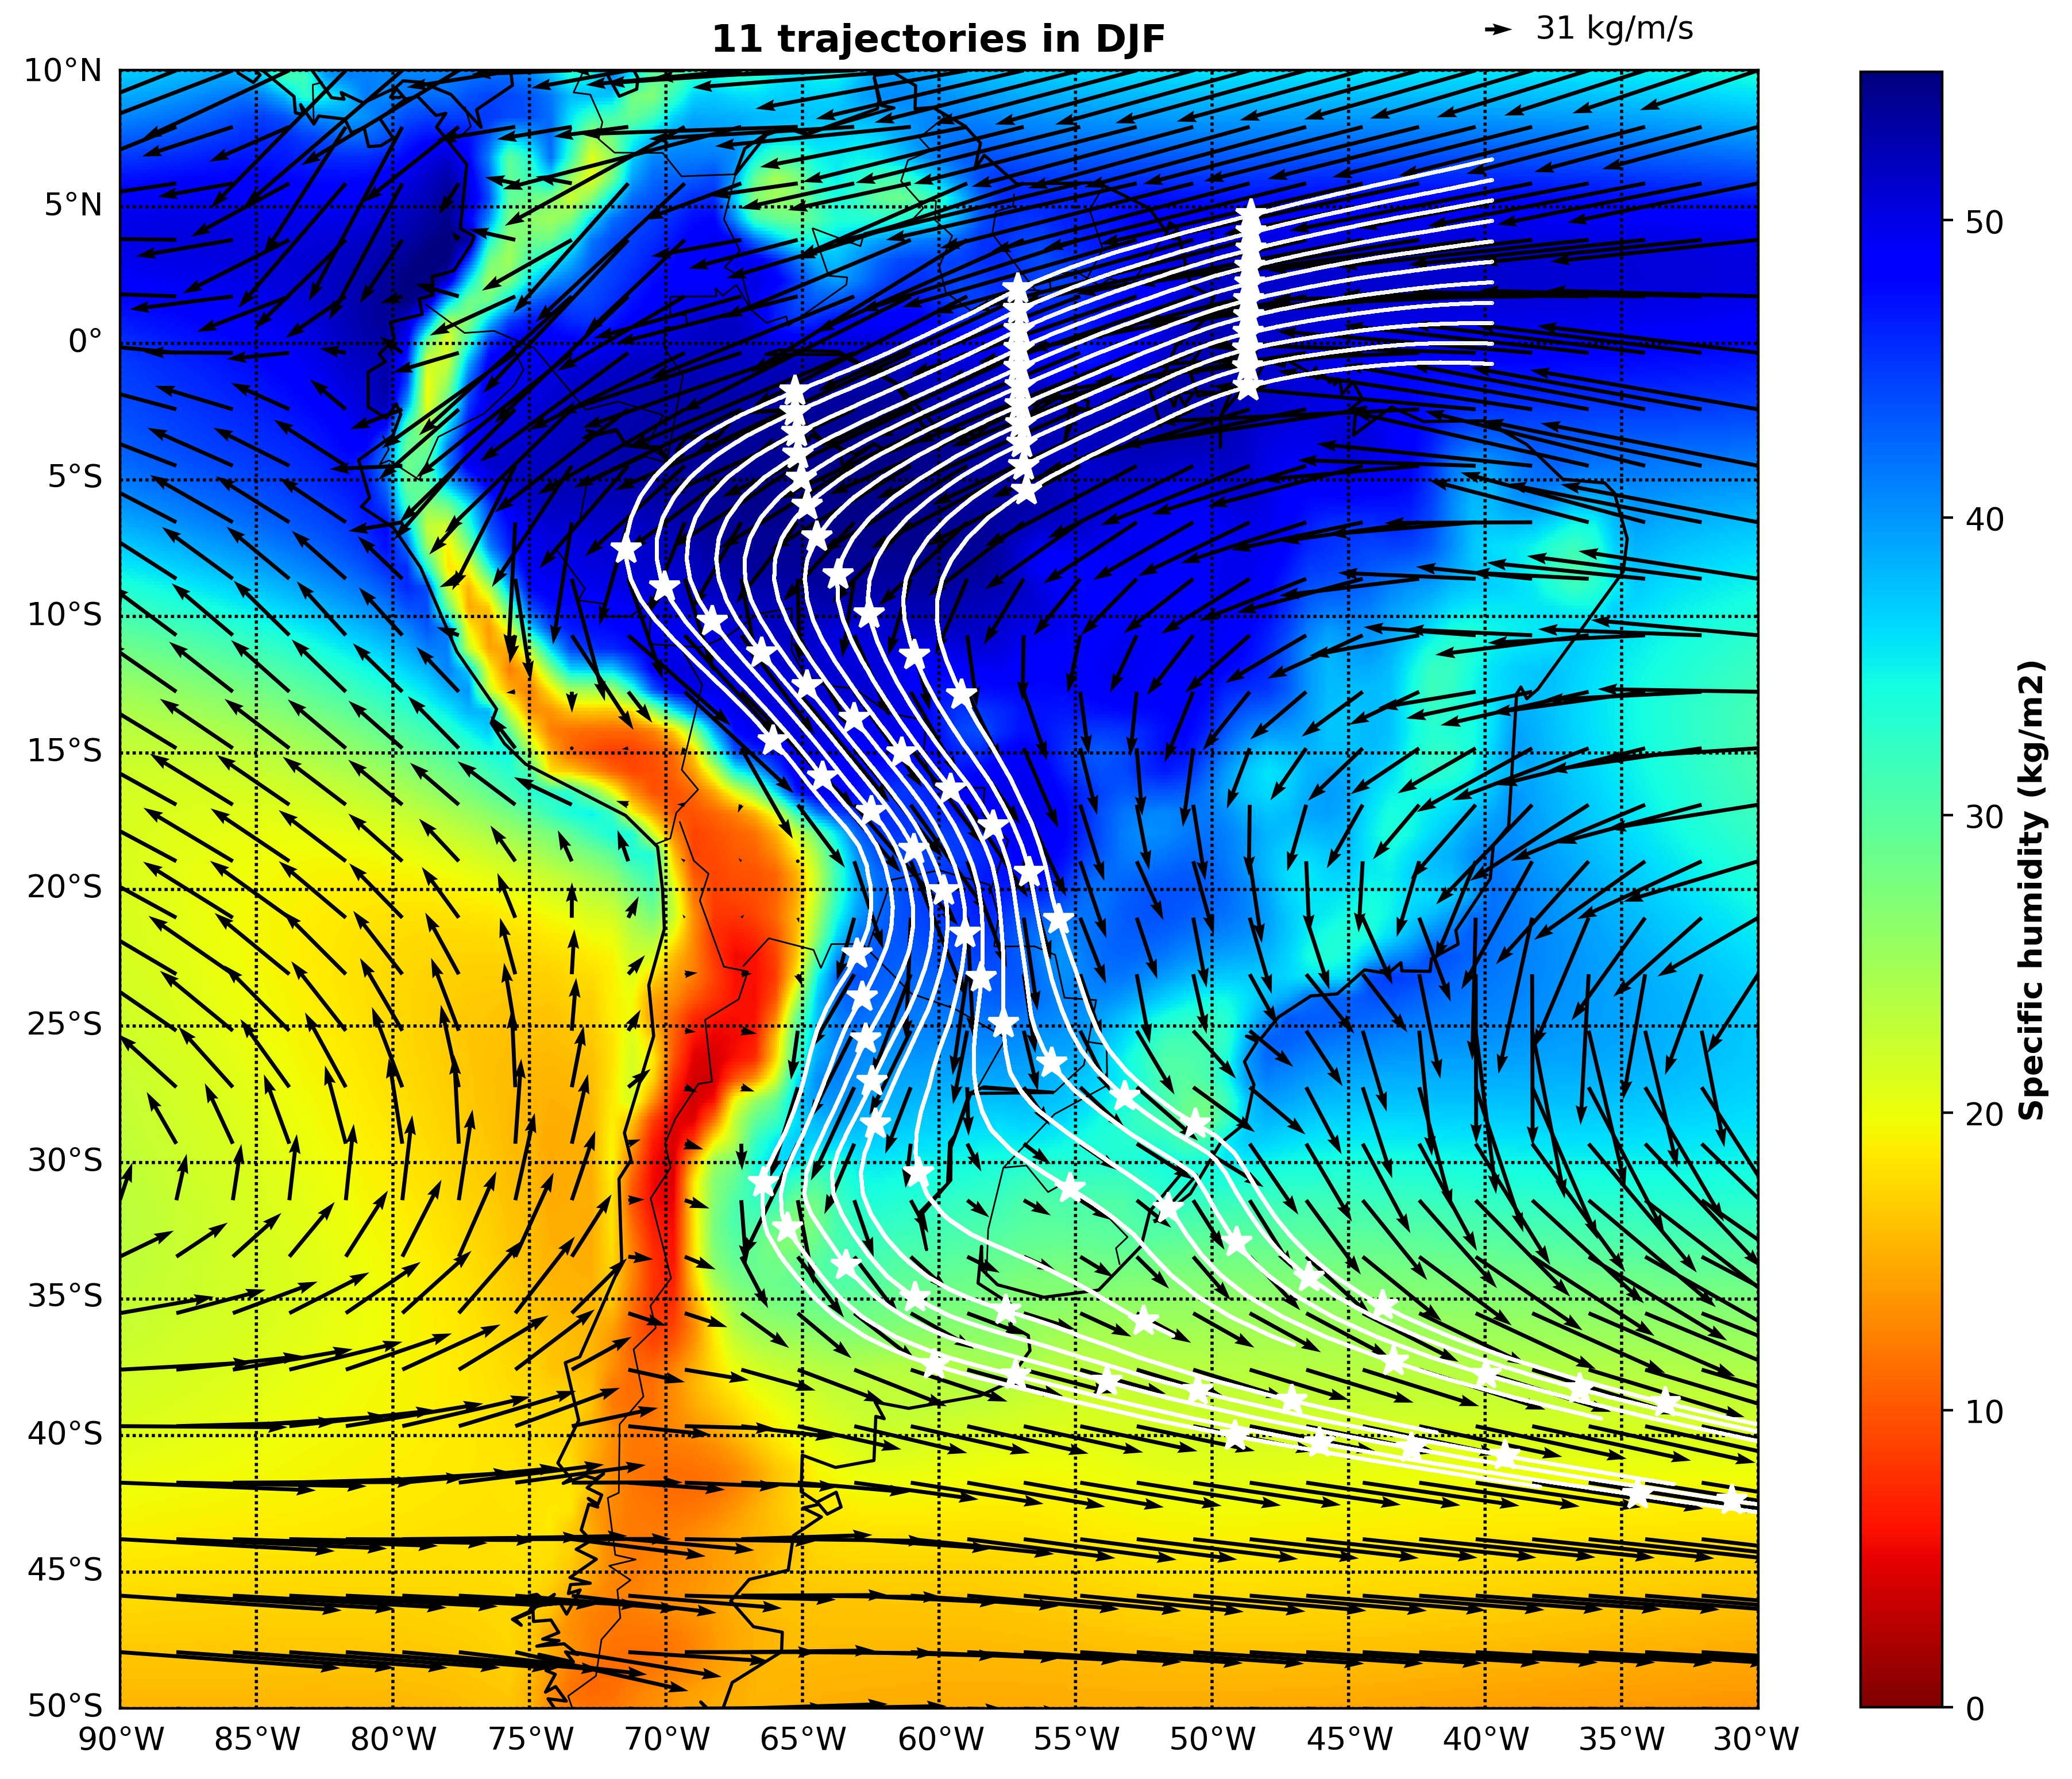
\includegraphics[width=0.70\linewidth]{DJF} \\
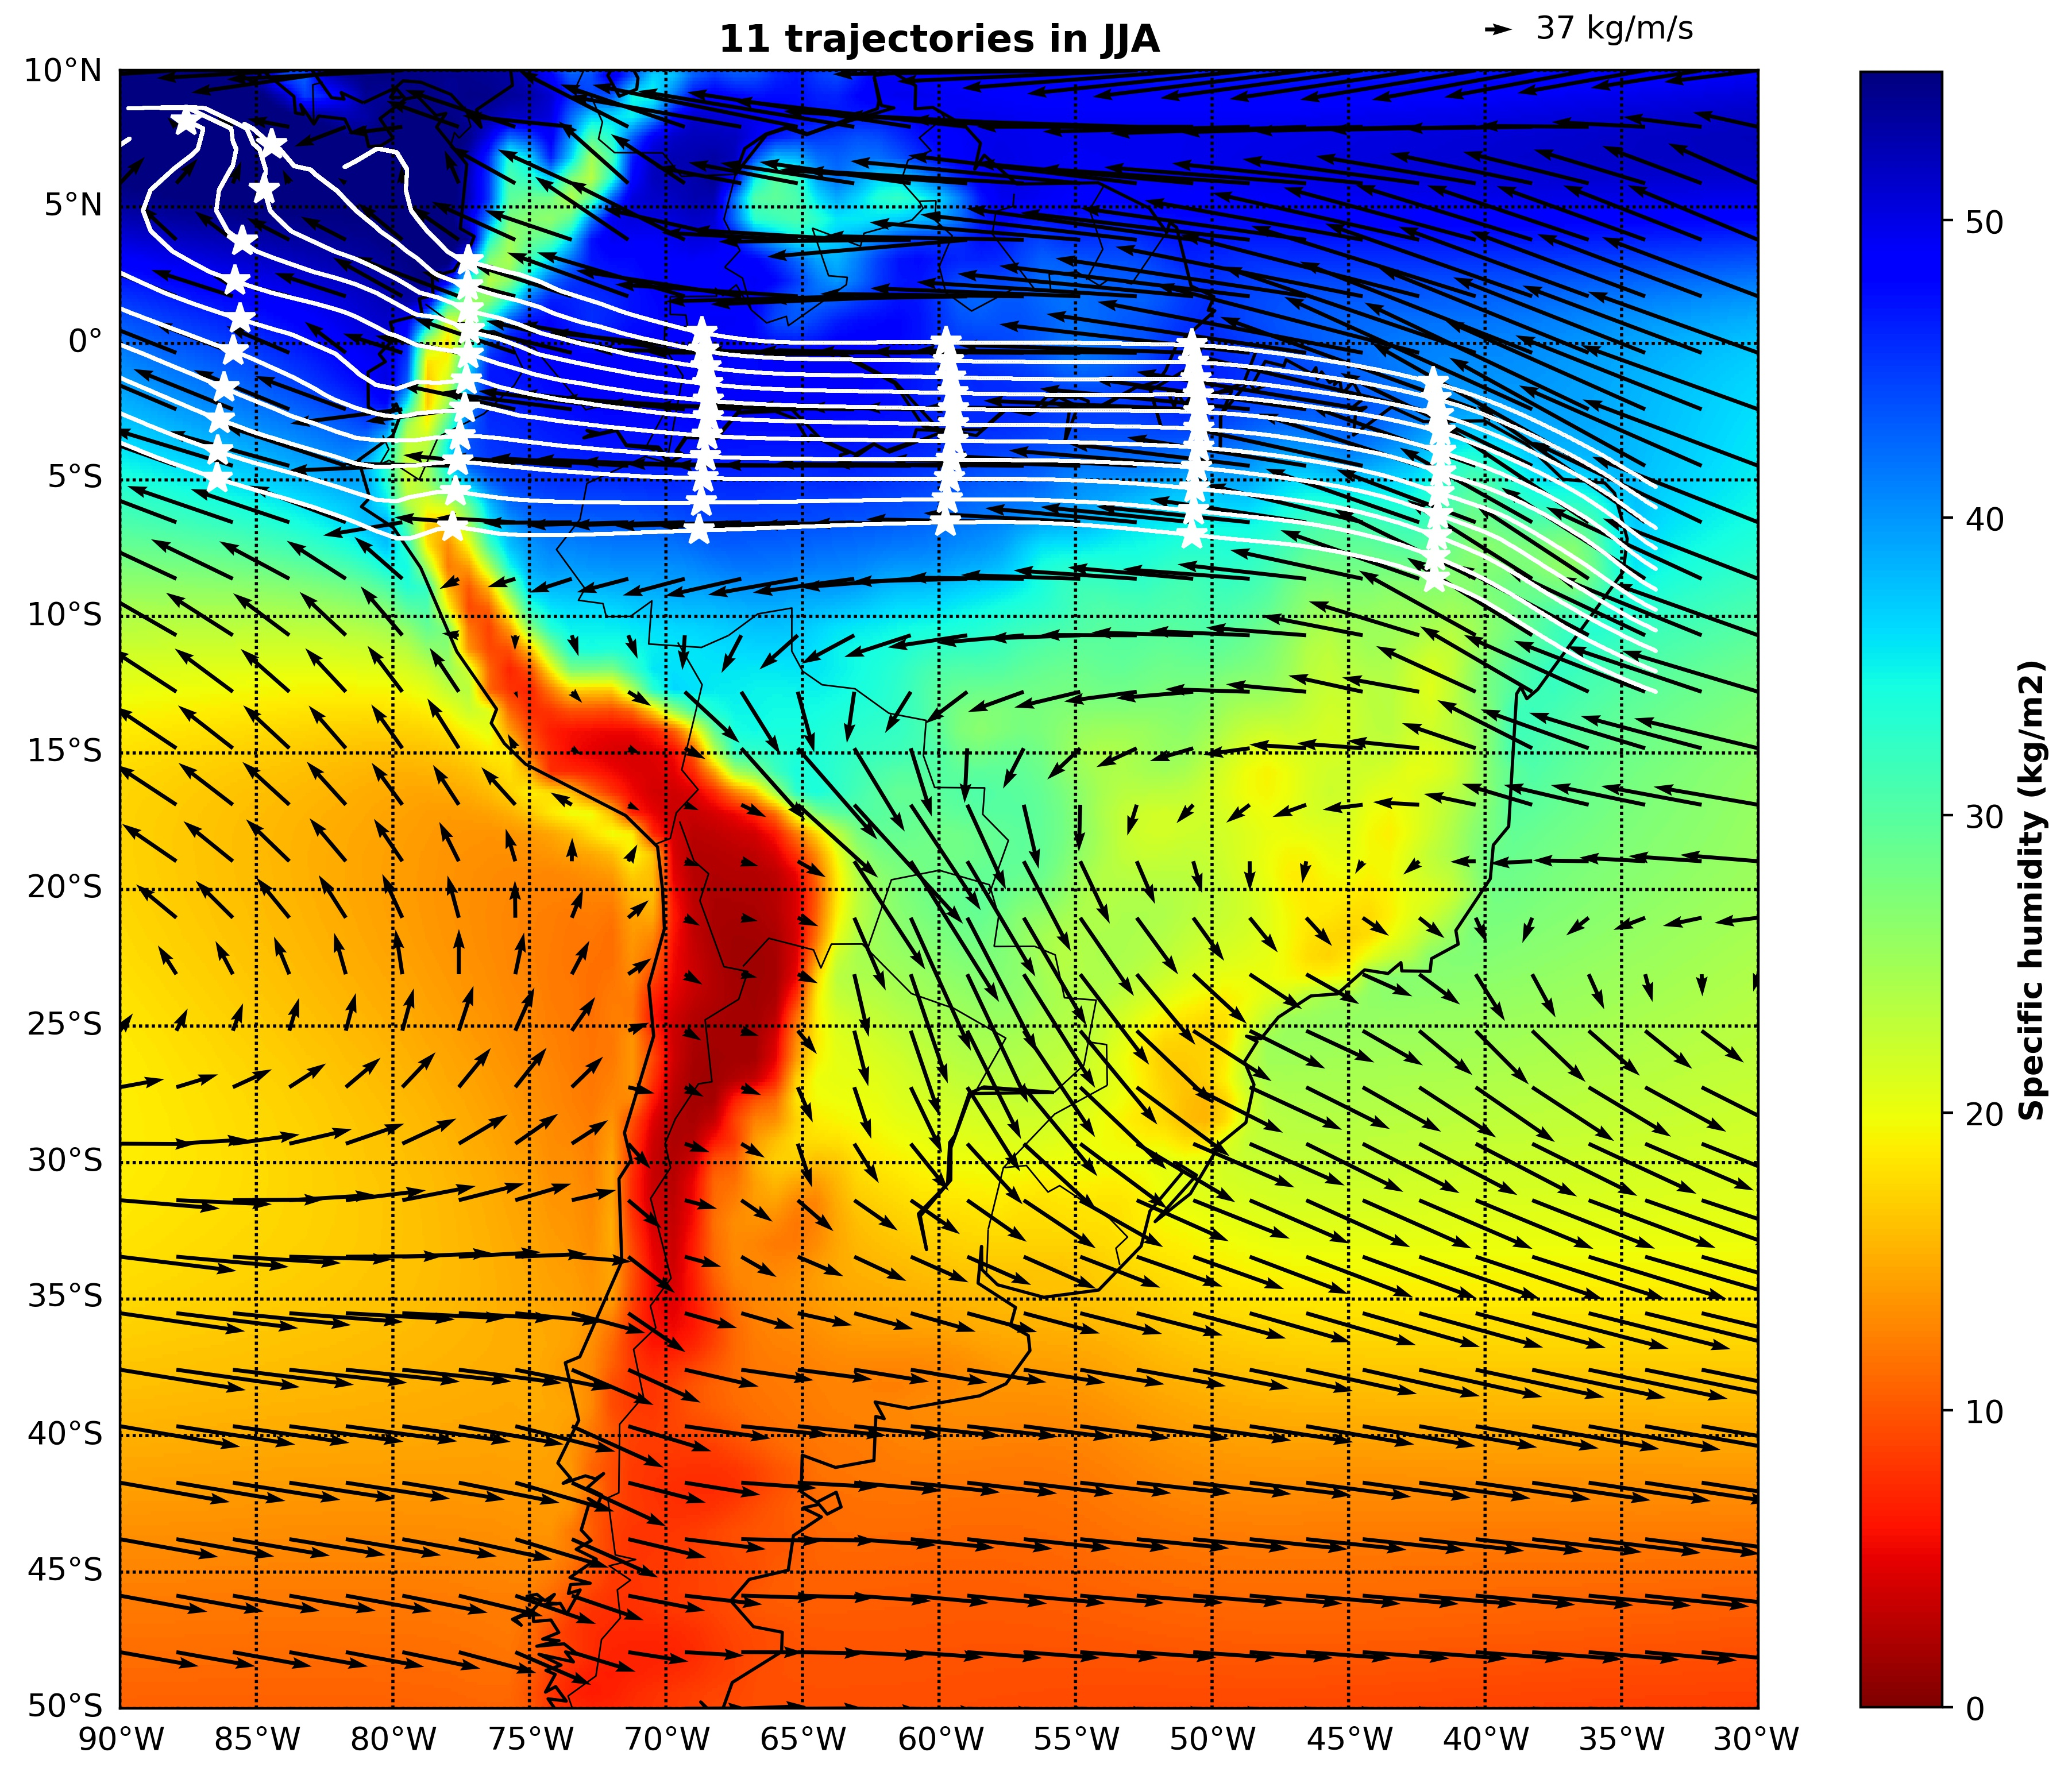
\includegraphics[width=0.70\linewidth]{JJA} 
\captionof{figure}{Examples of moisture flux trajectories represented by white
lines. The white stars mark traveled distances of 1,000 km. The first figure shows
the results for summer, and the second one for winter.}
\end{center}\vspace{0.5cm}

\begin{center}
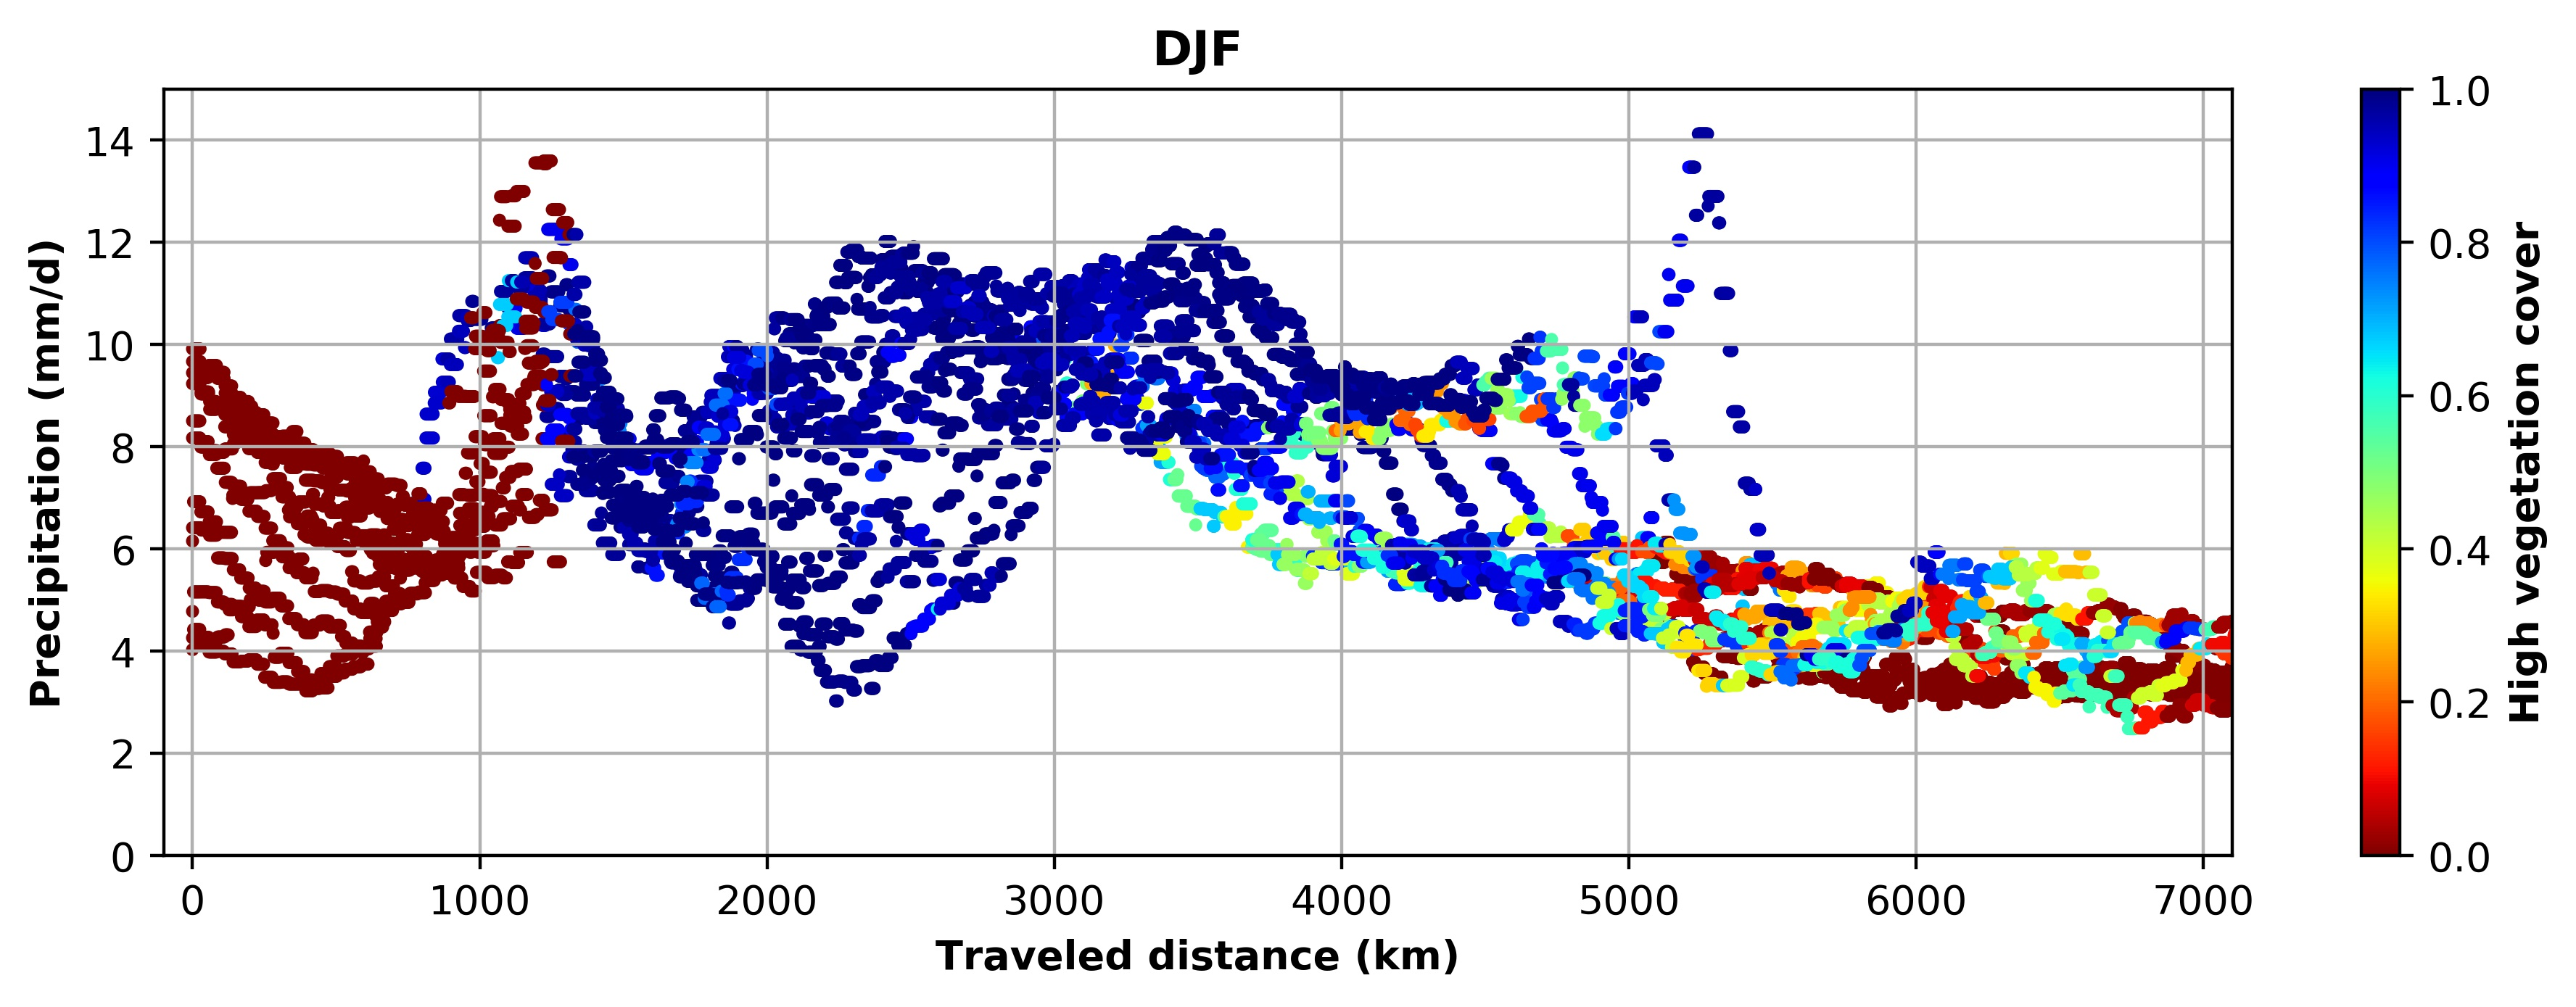
\includegraphics[width=0.49\linewidth]{PCPDJF} 
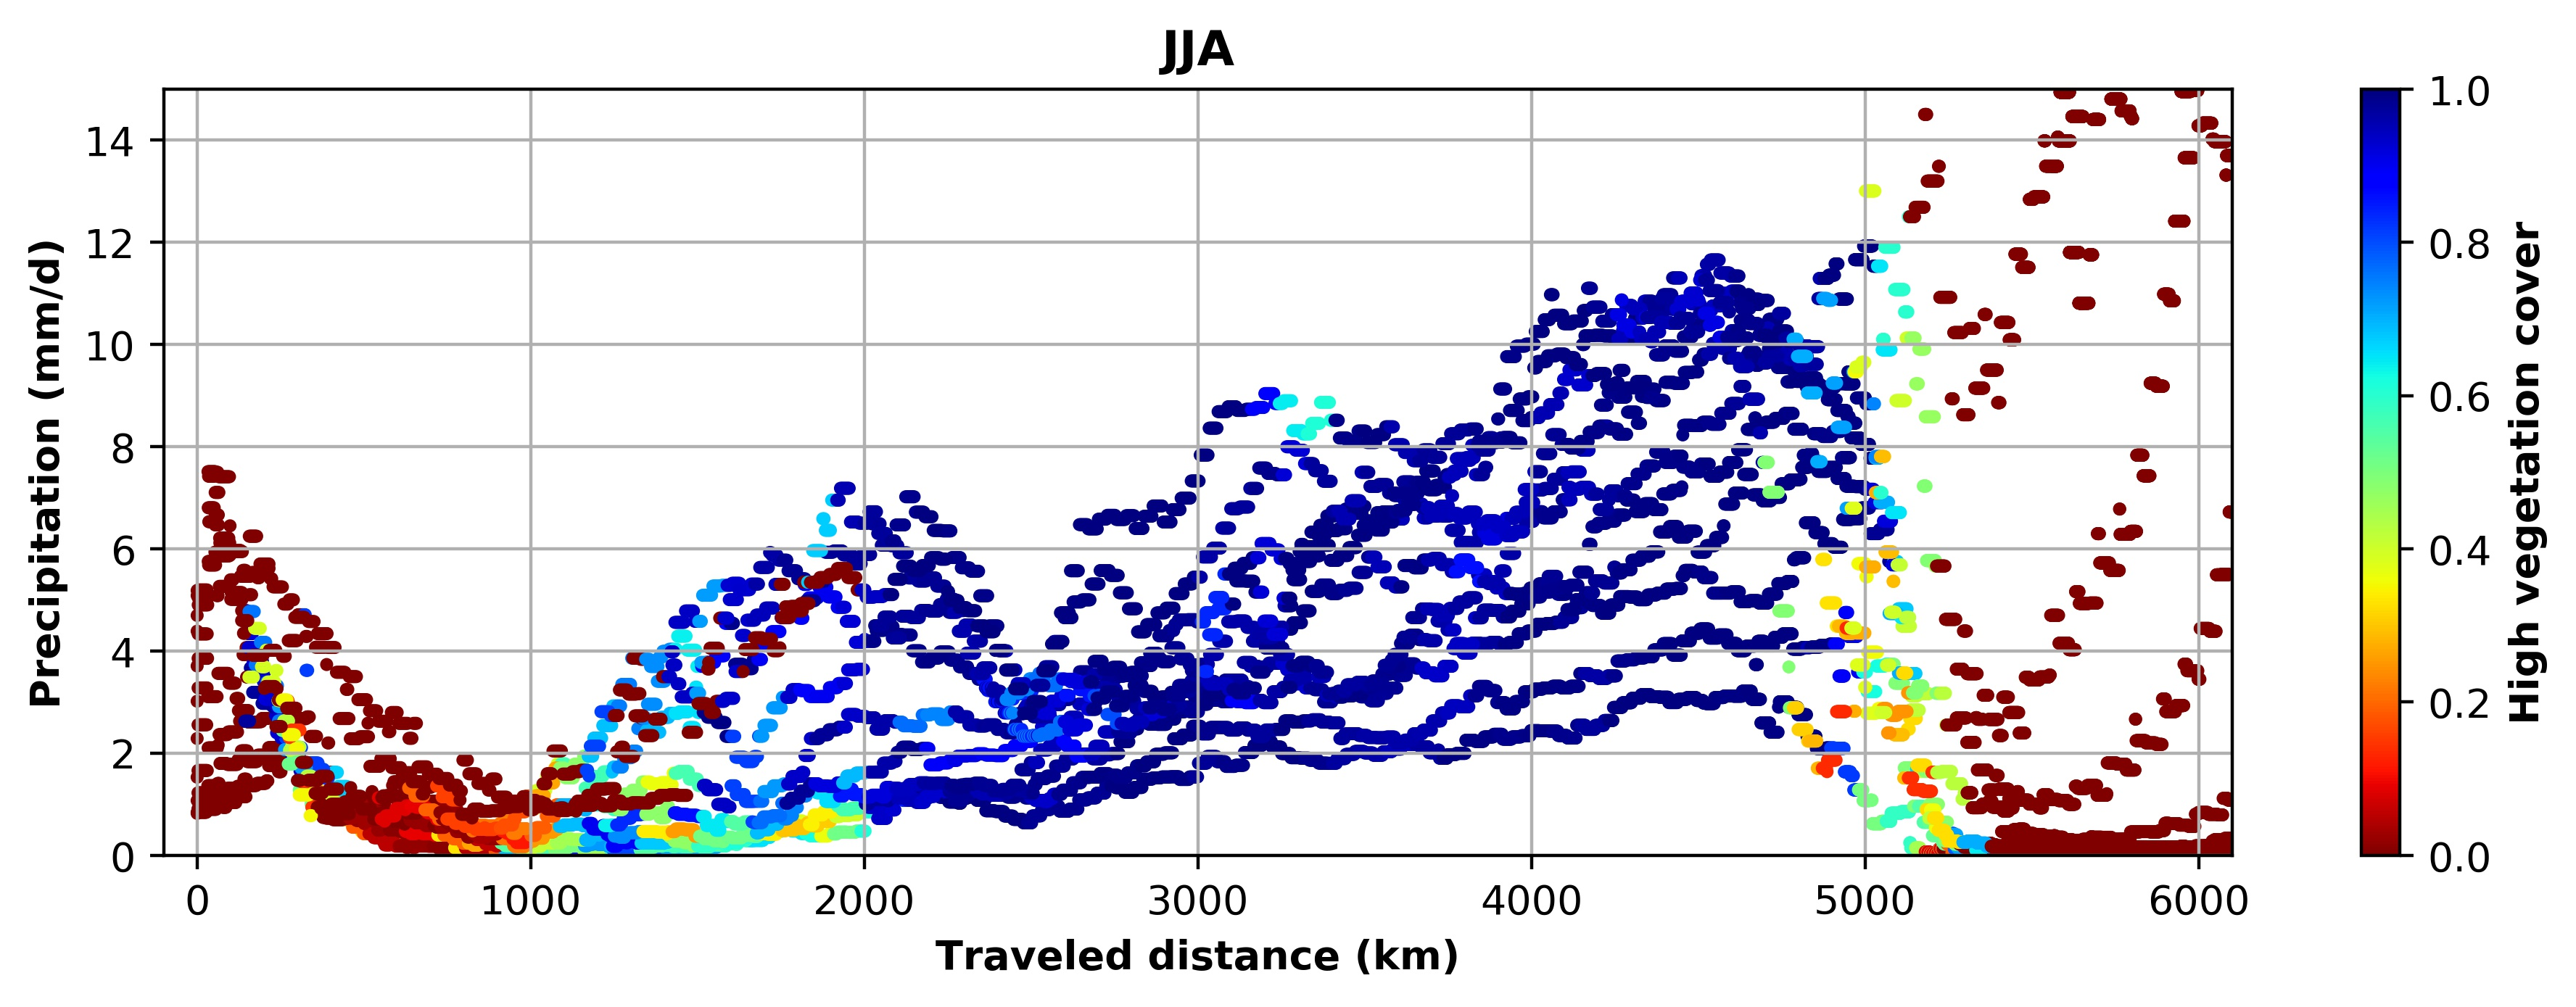
\includegraphics[width=0.49\linewidth]{PCPJJA} \\
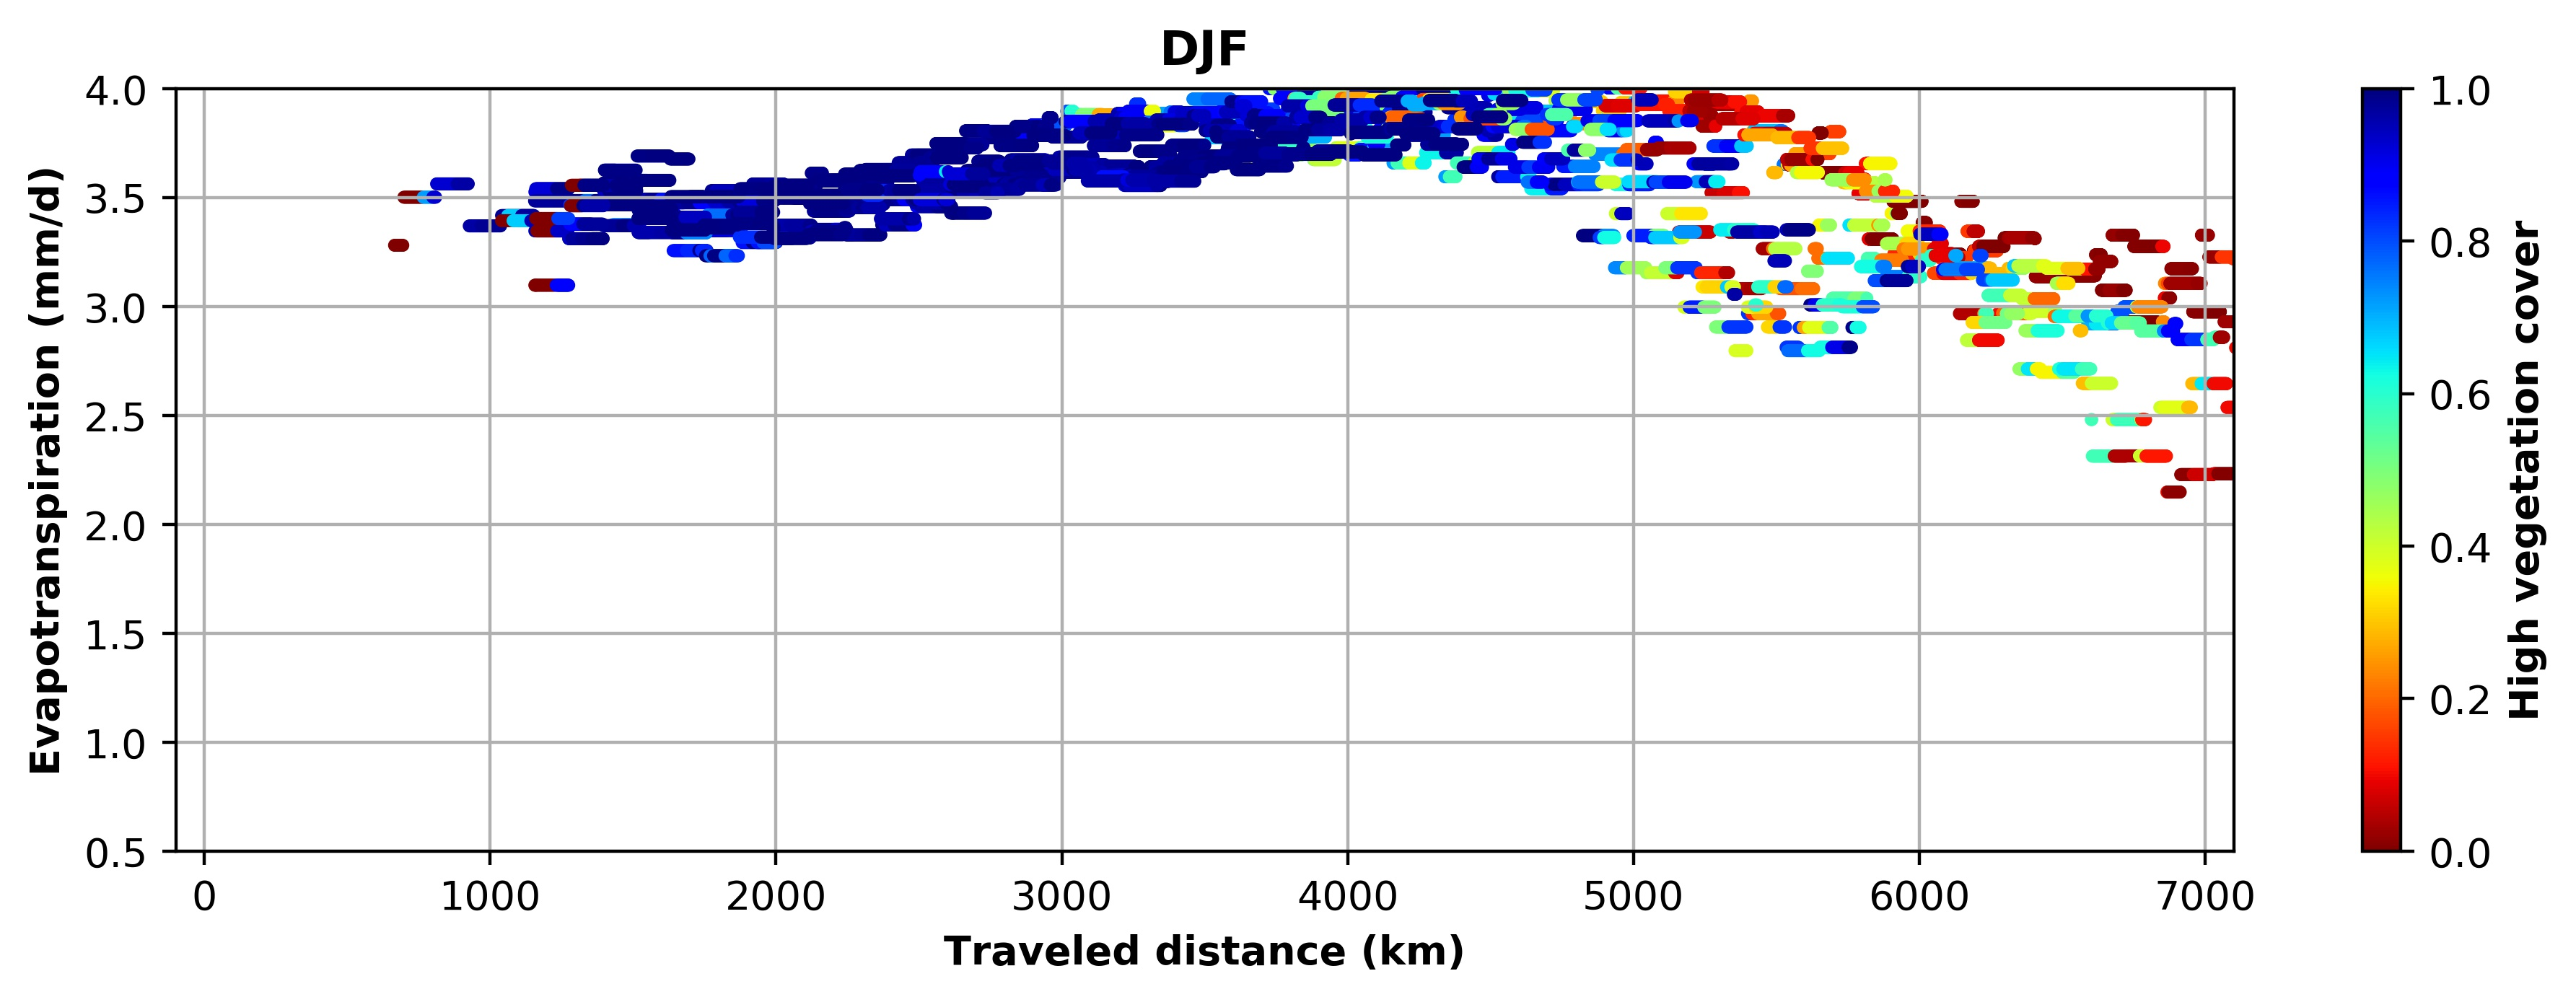
\includegraphics[width=0.49\linewidth]{ETDJF} 
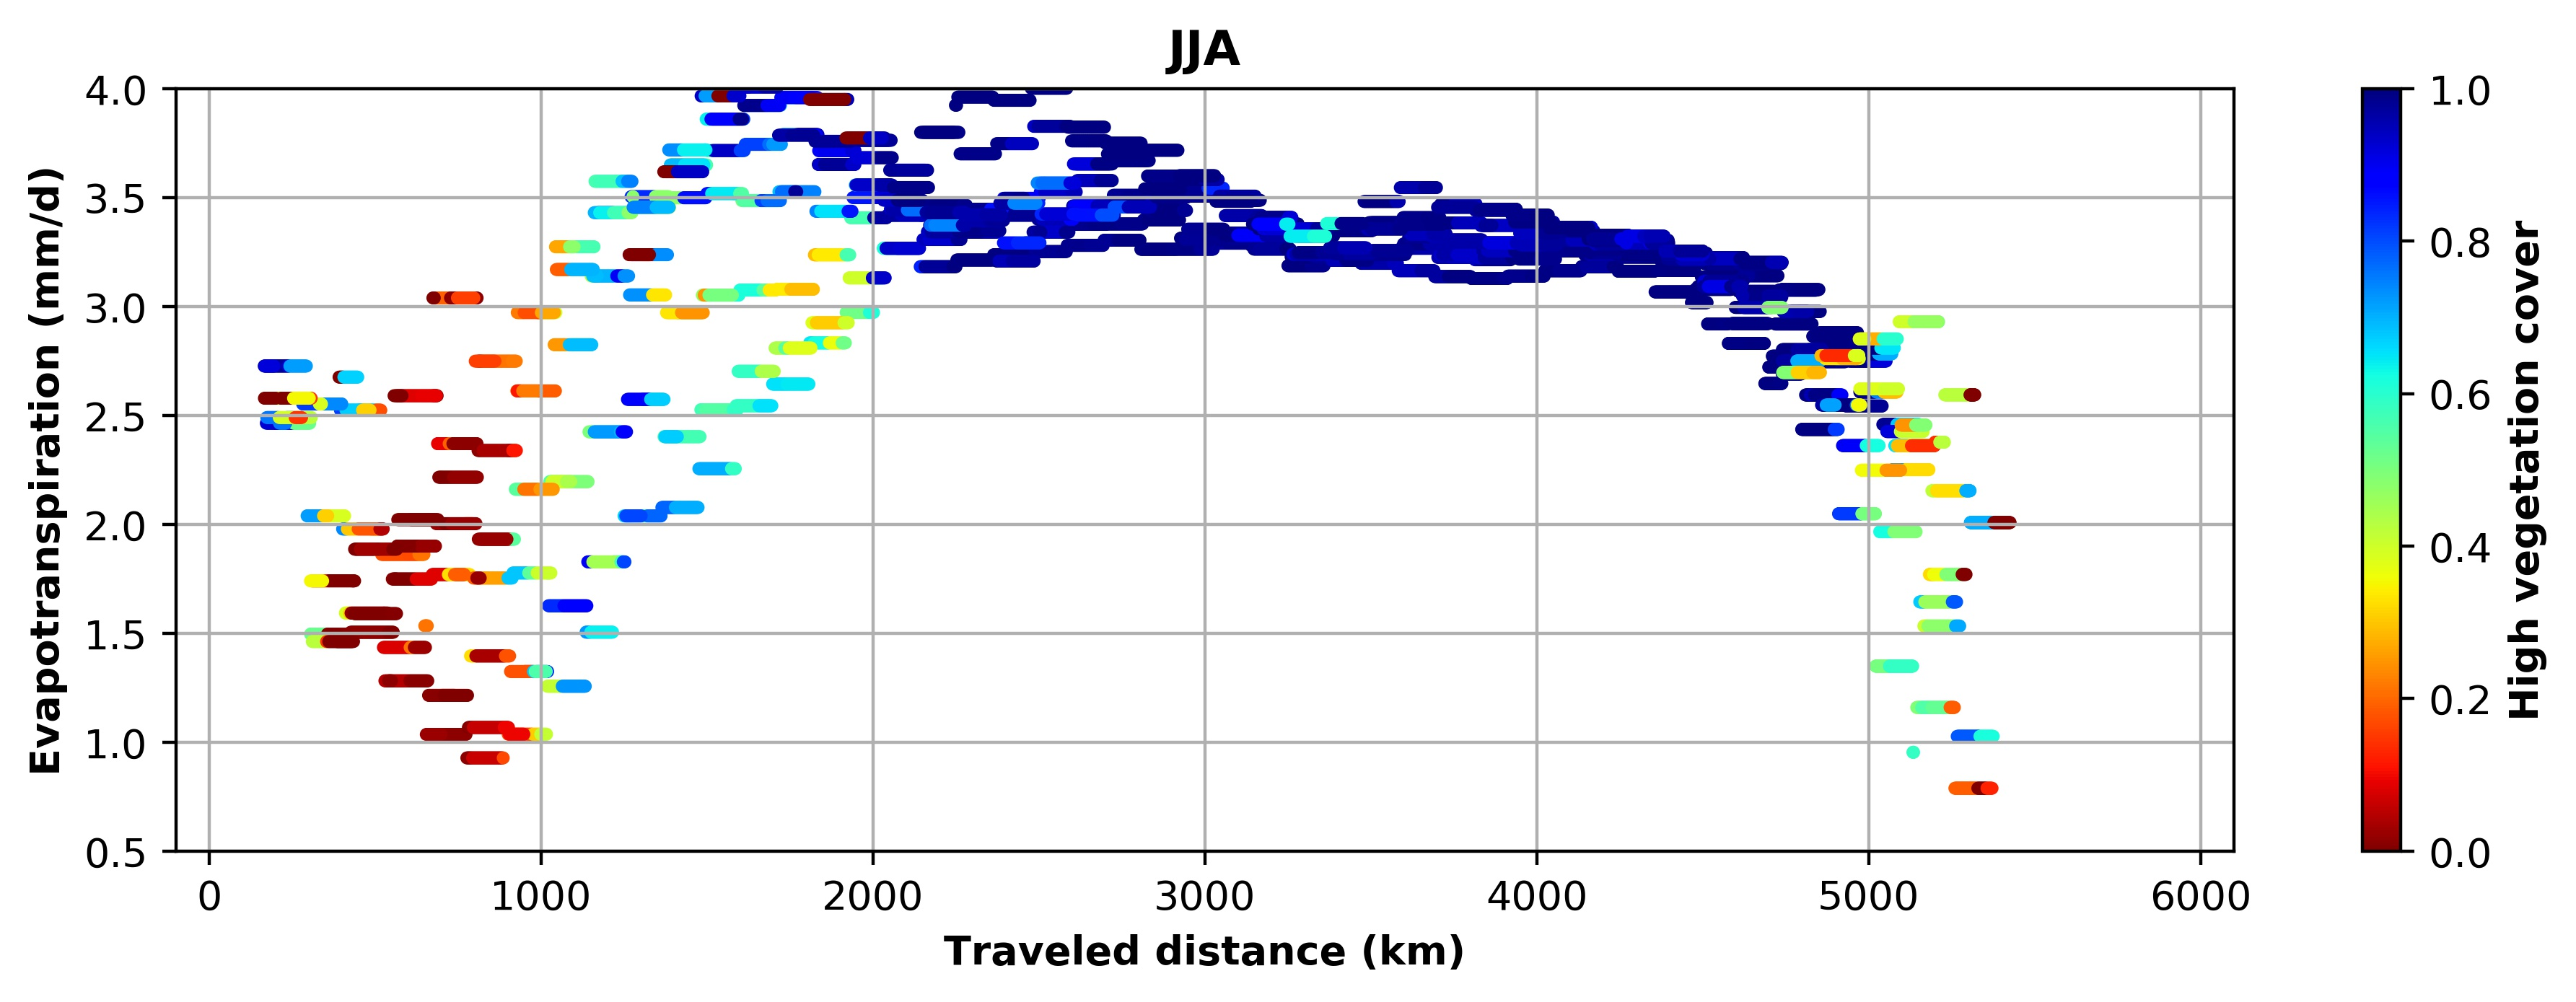
\includegraphics[width=0.49\linewidth]{ETJJA} \\
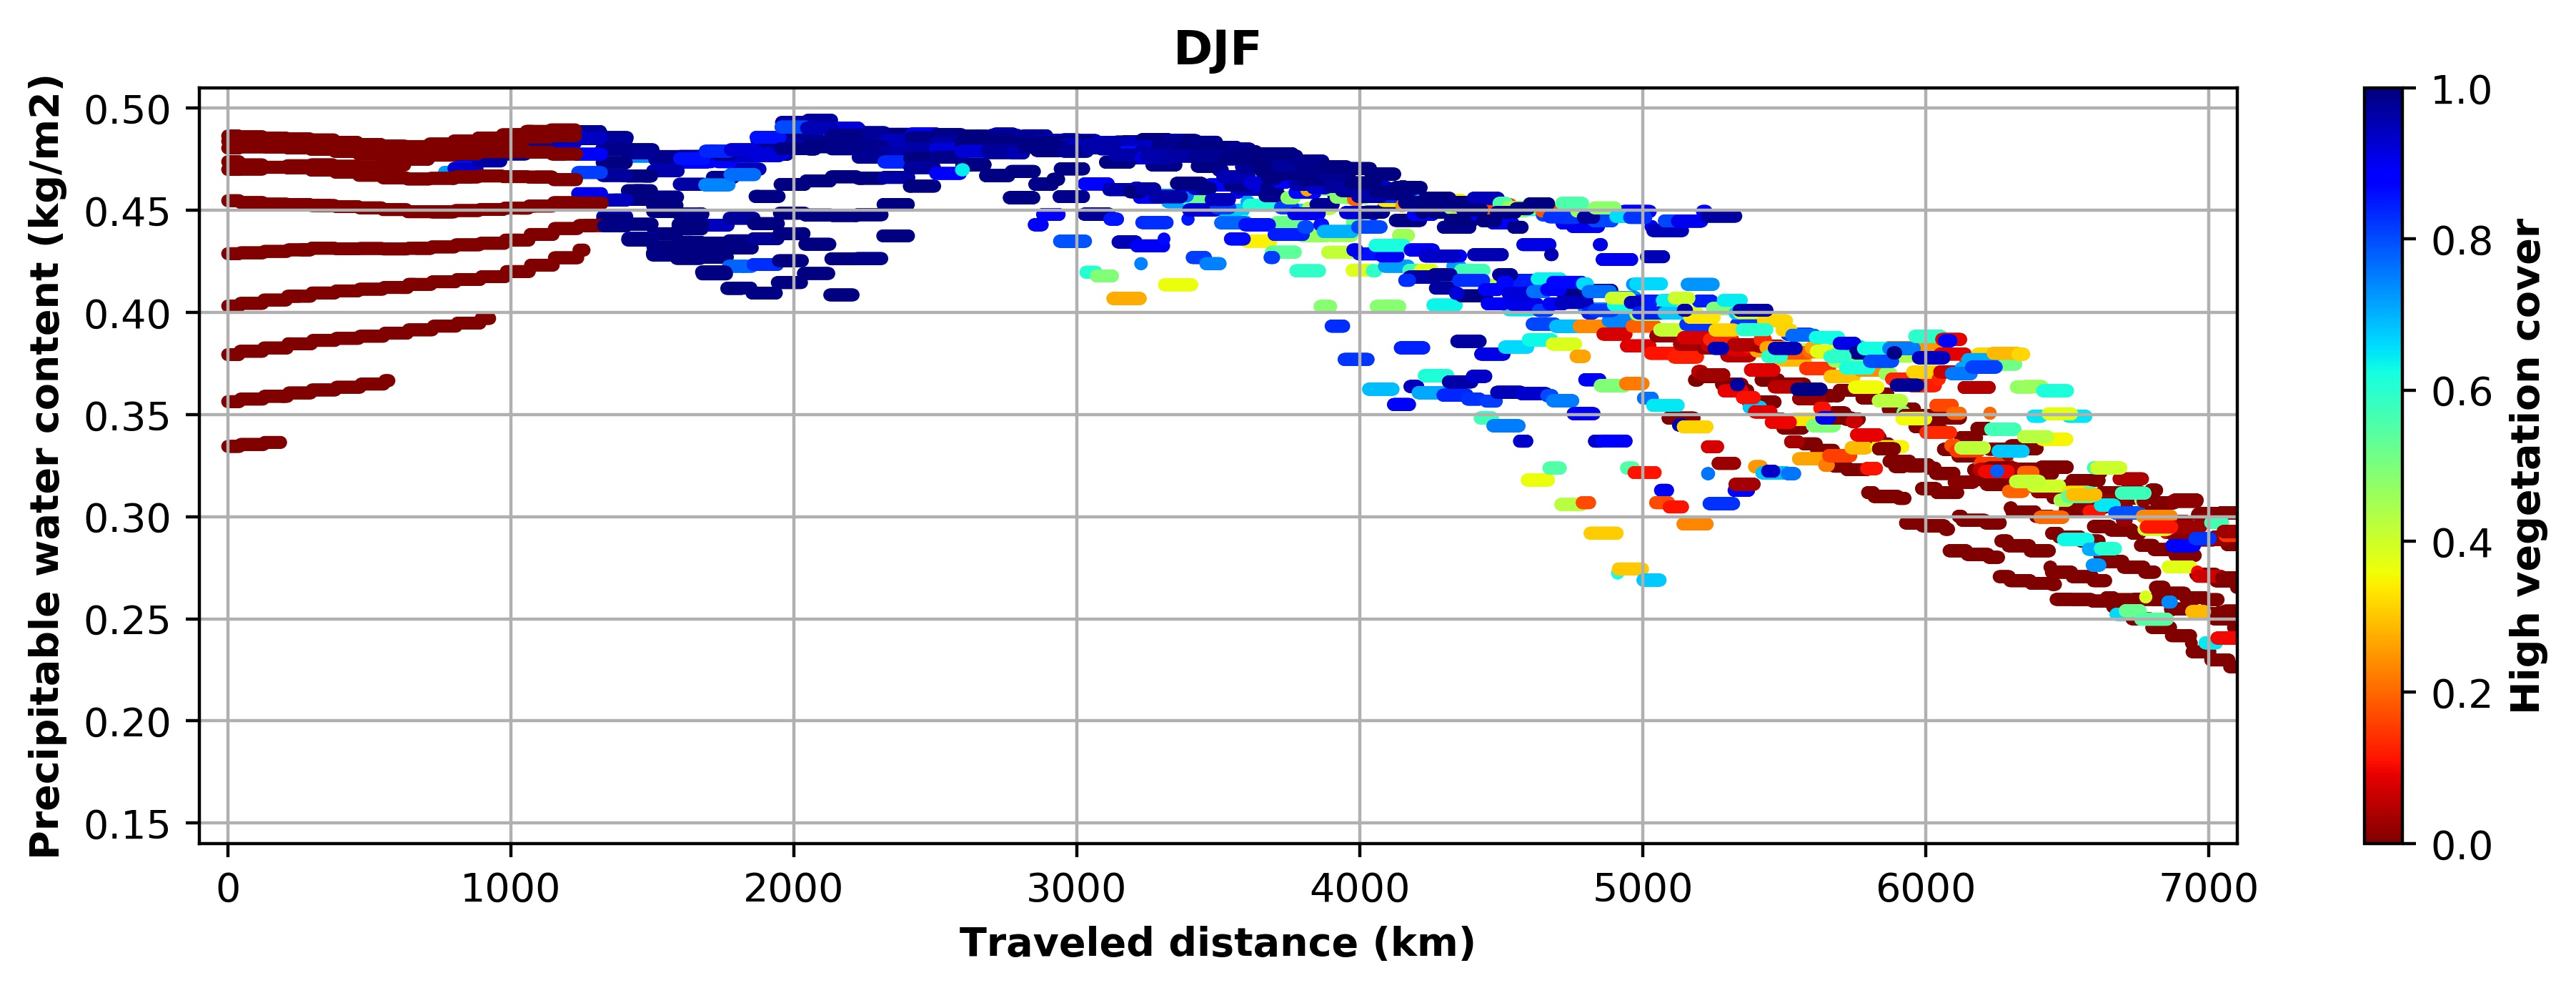
\includegraphics[width=0.49\linewidth]{PWCDJF} 
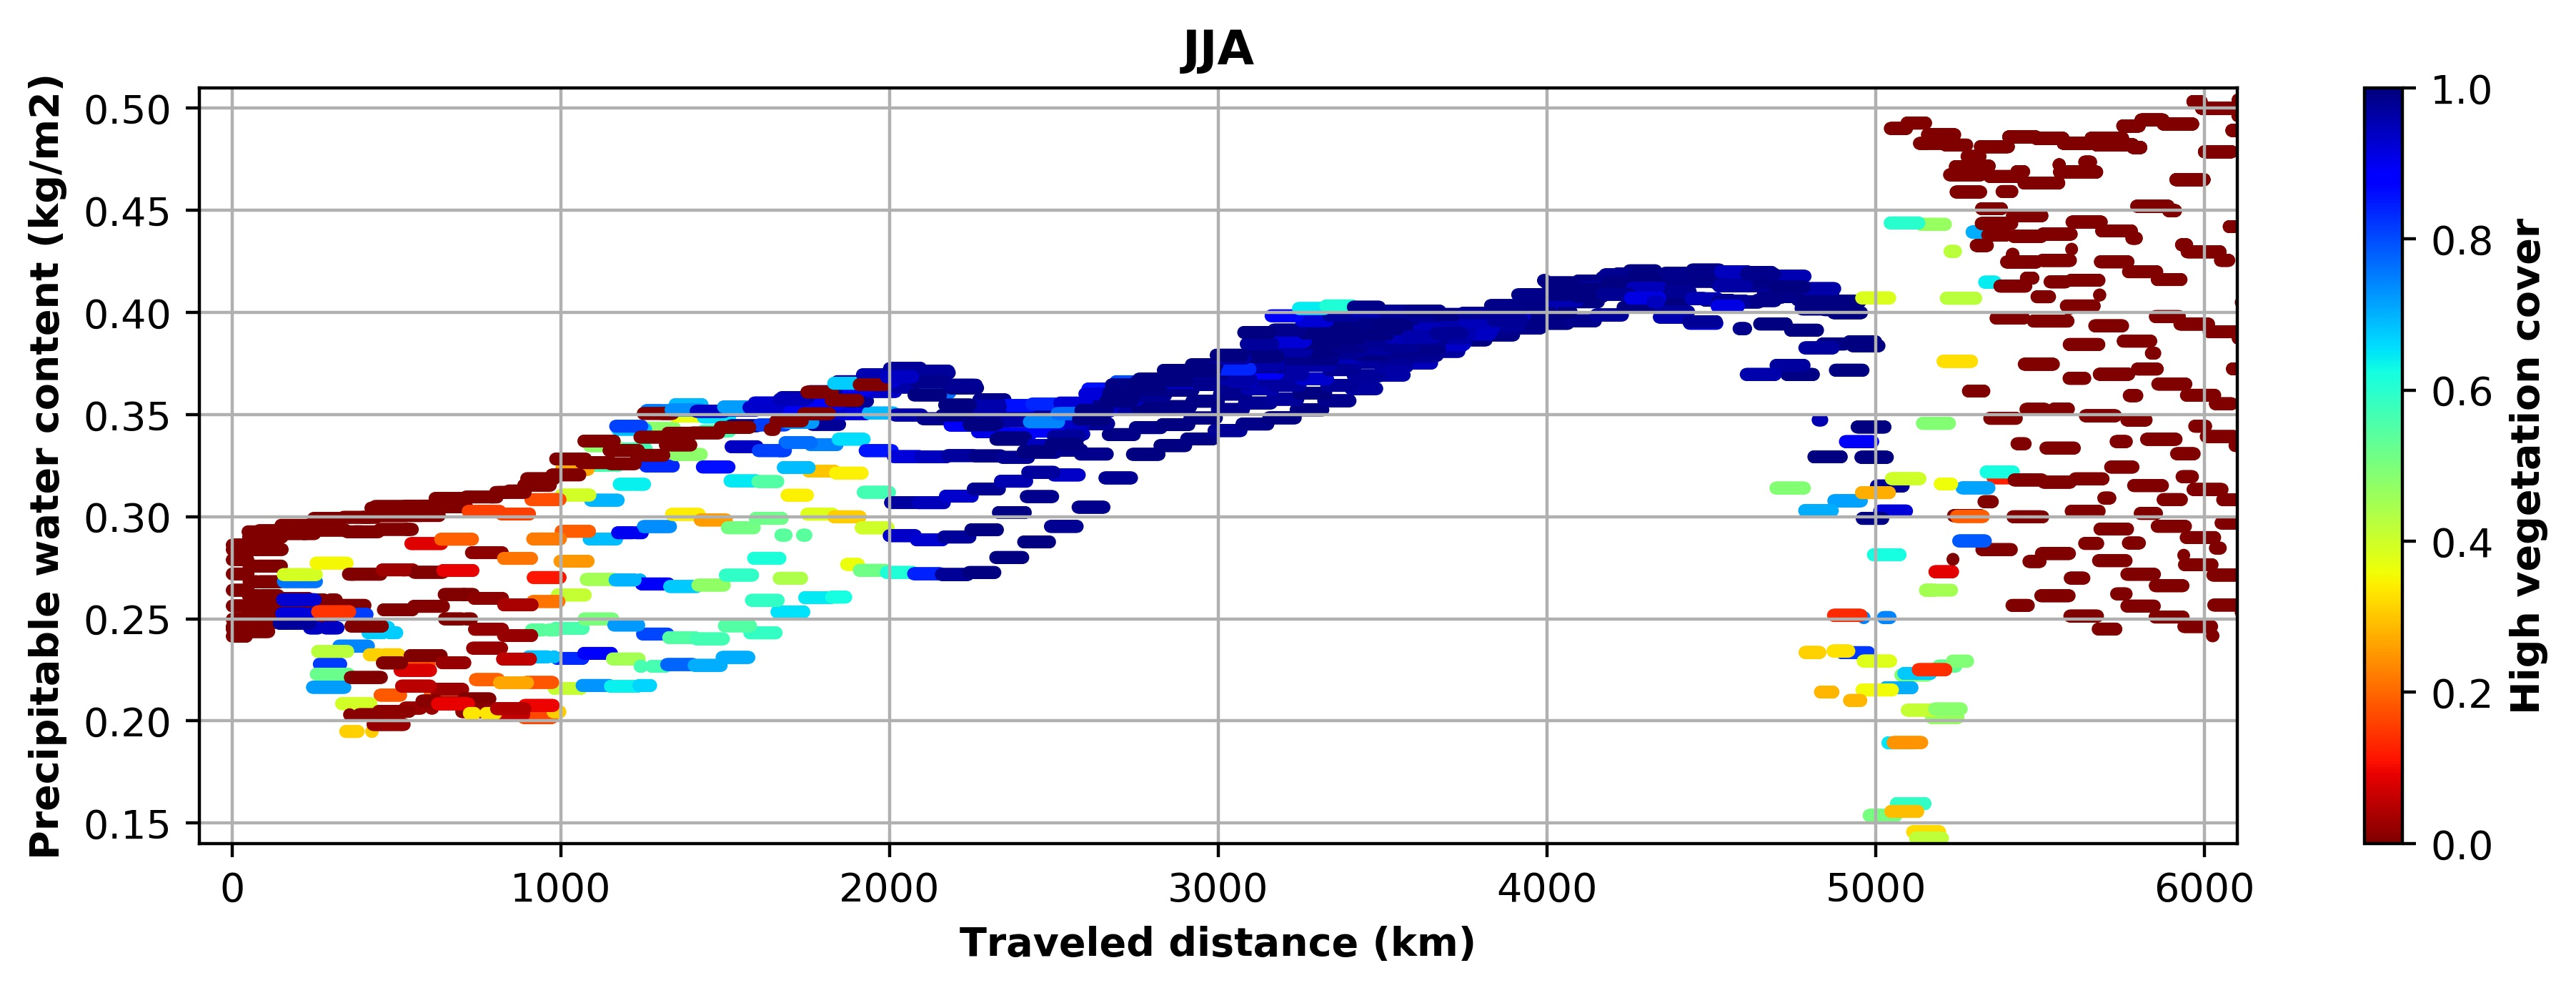
\includegraphics[width=0.49\linewidth]{PWCJJA} \\ 
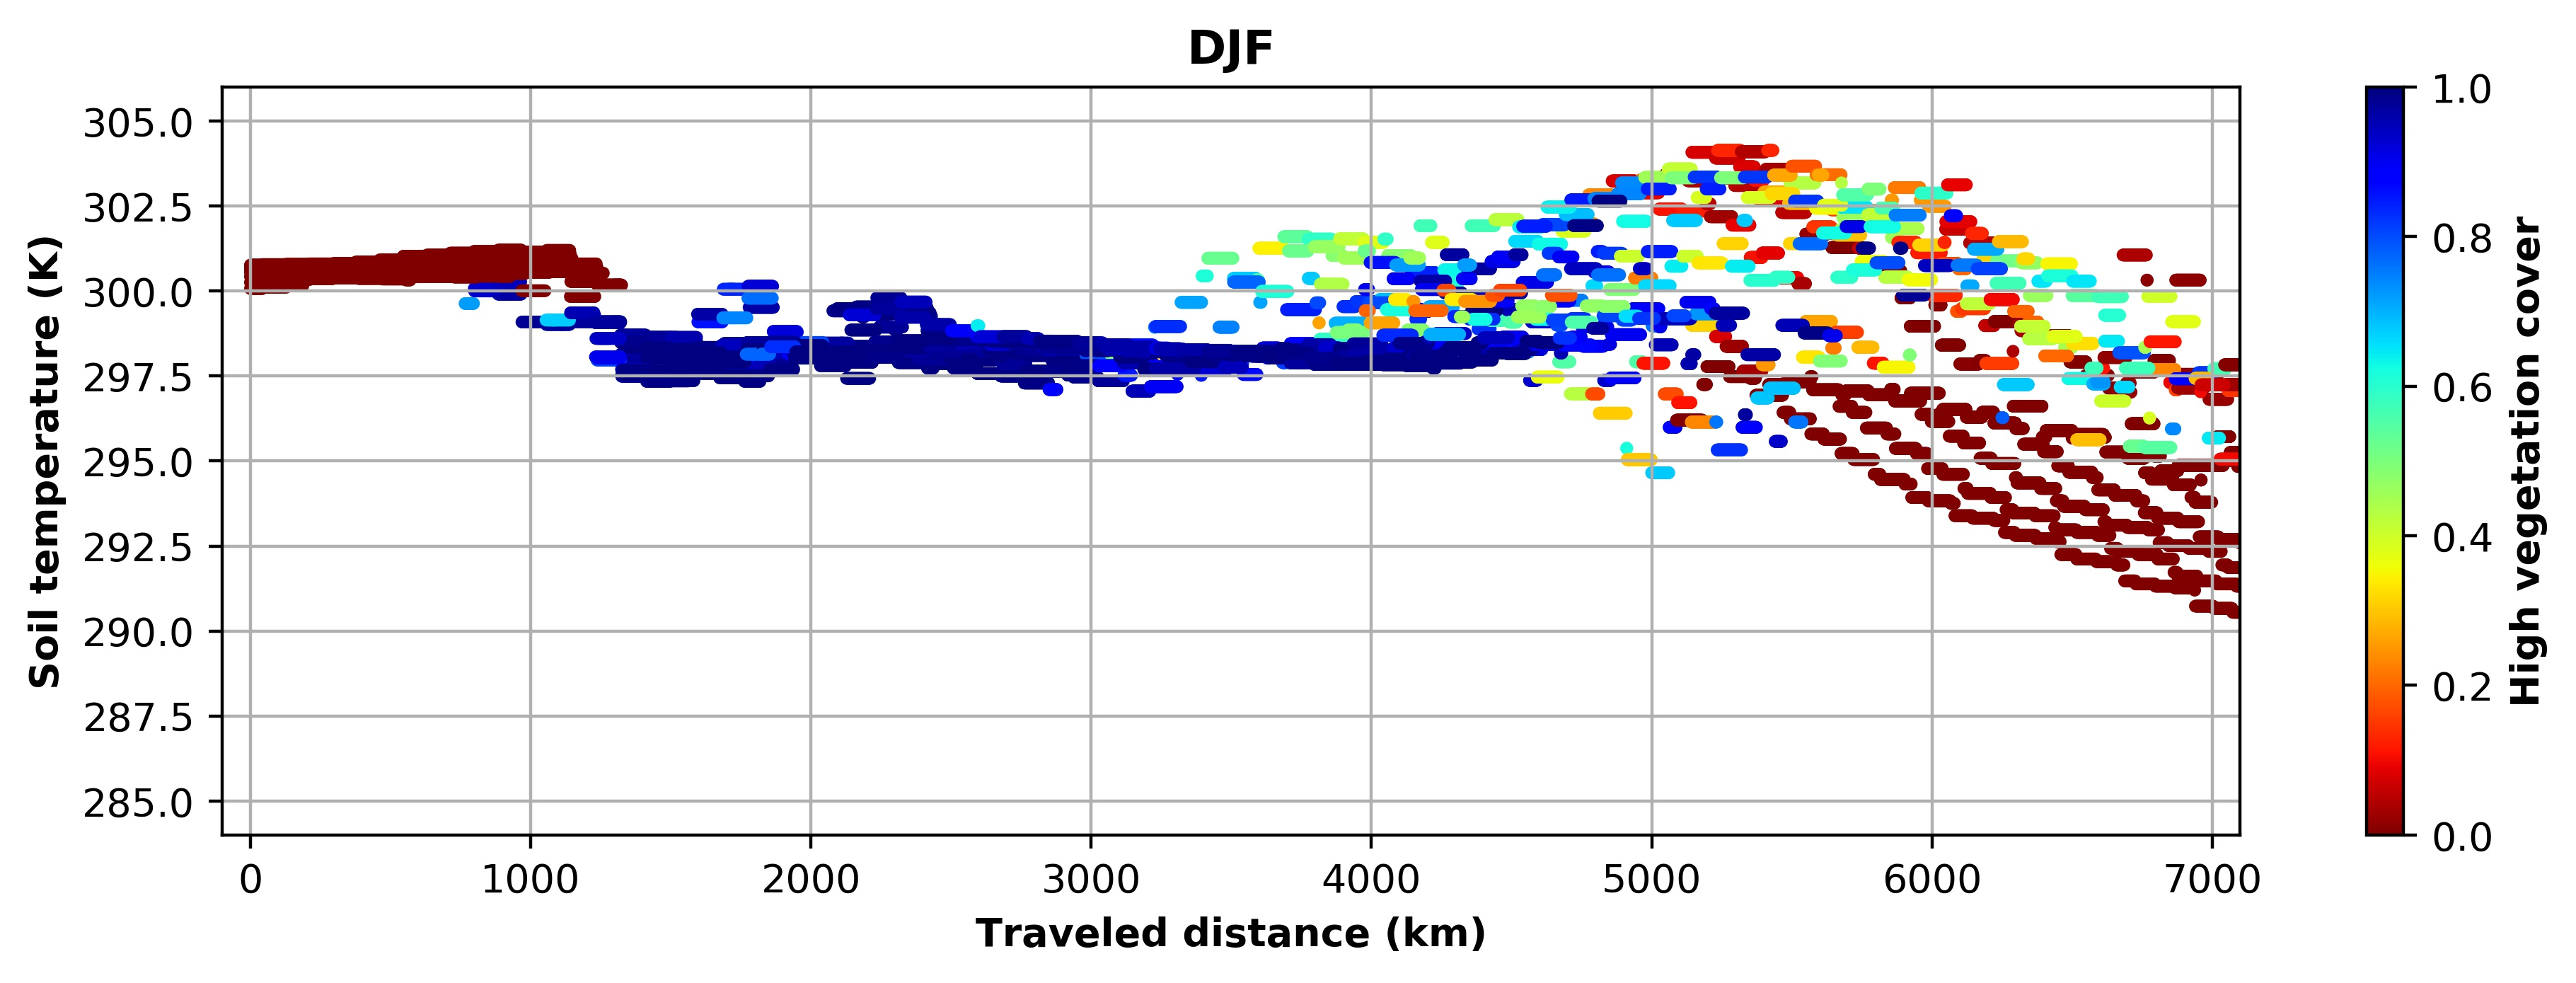
\includegraphics[width=0.49\linewidth]{STDJF} 
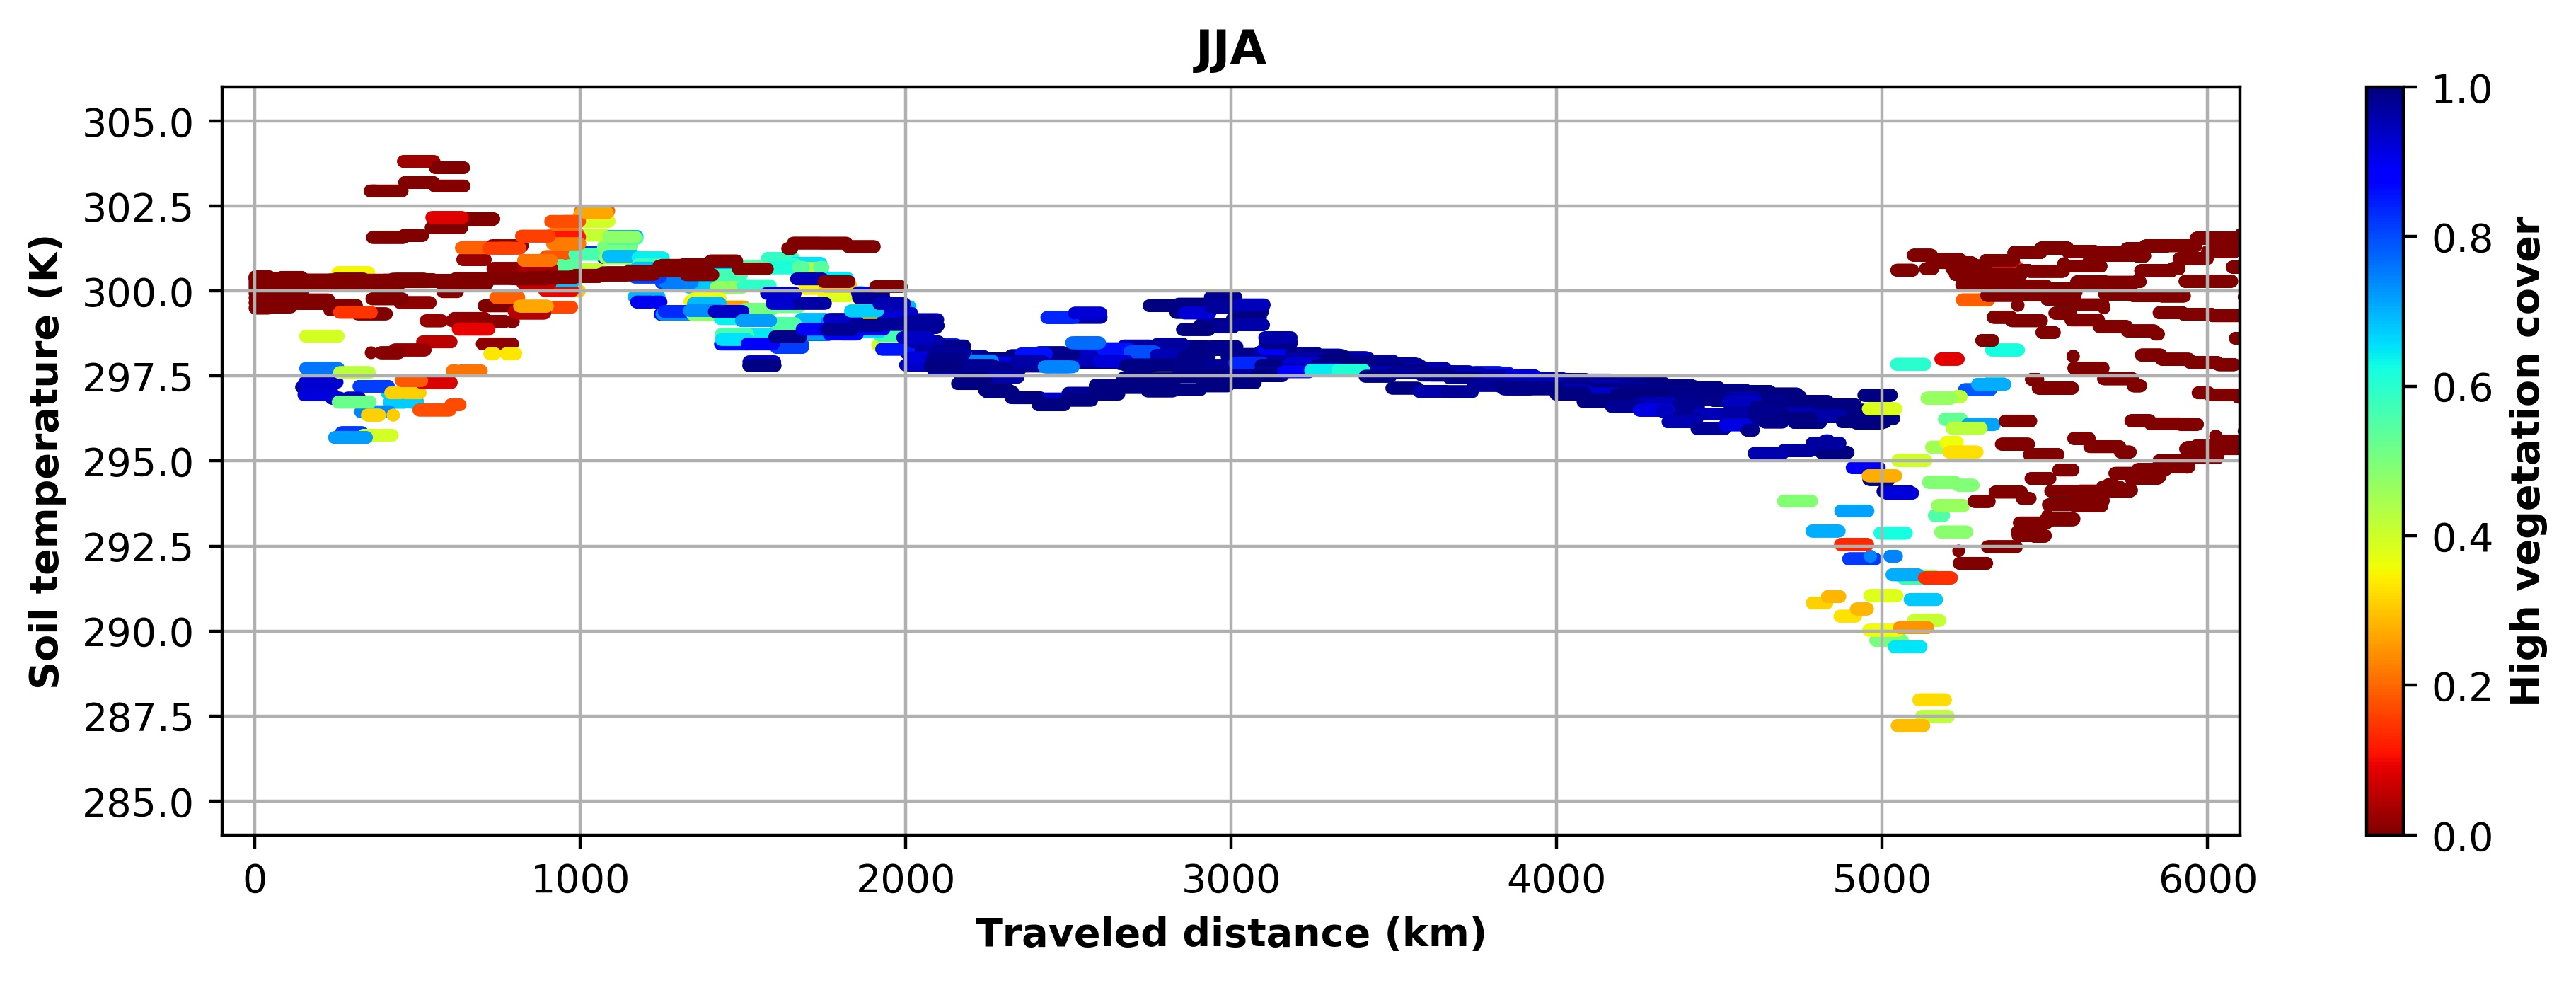
\includegraphics[width=0.49\linewidth]{STJJA} \\
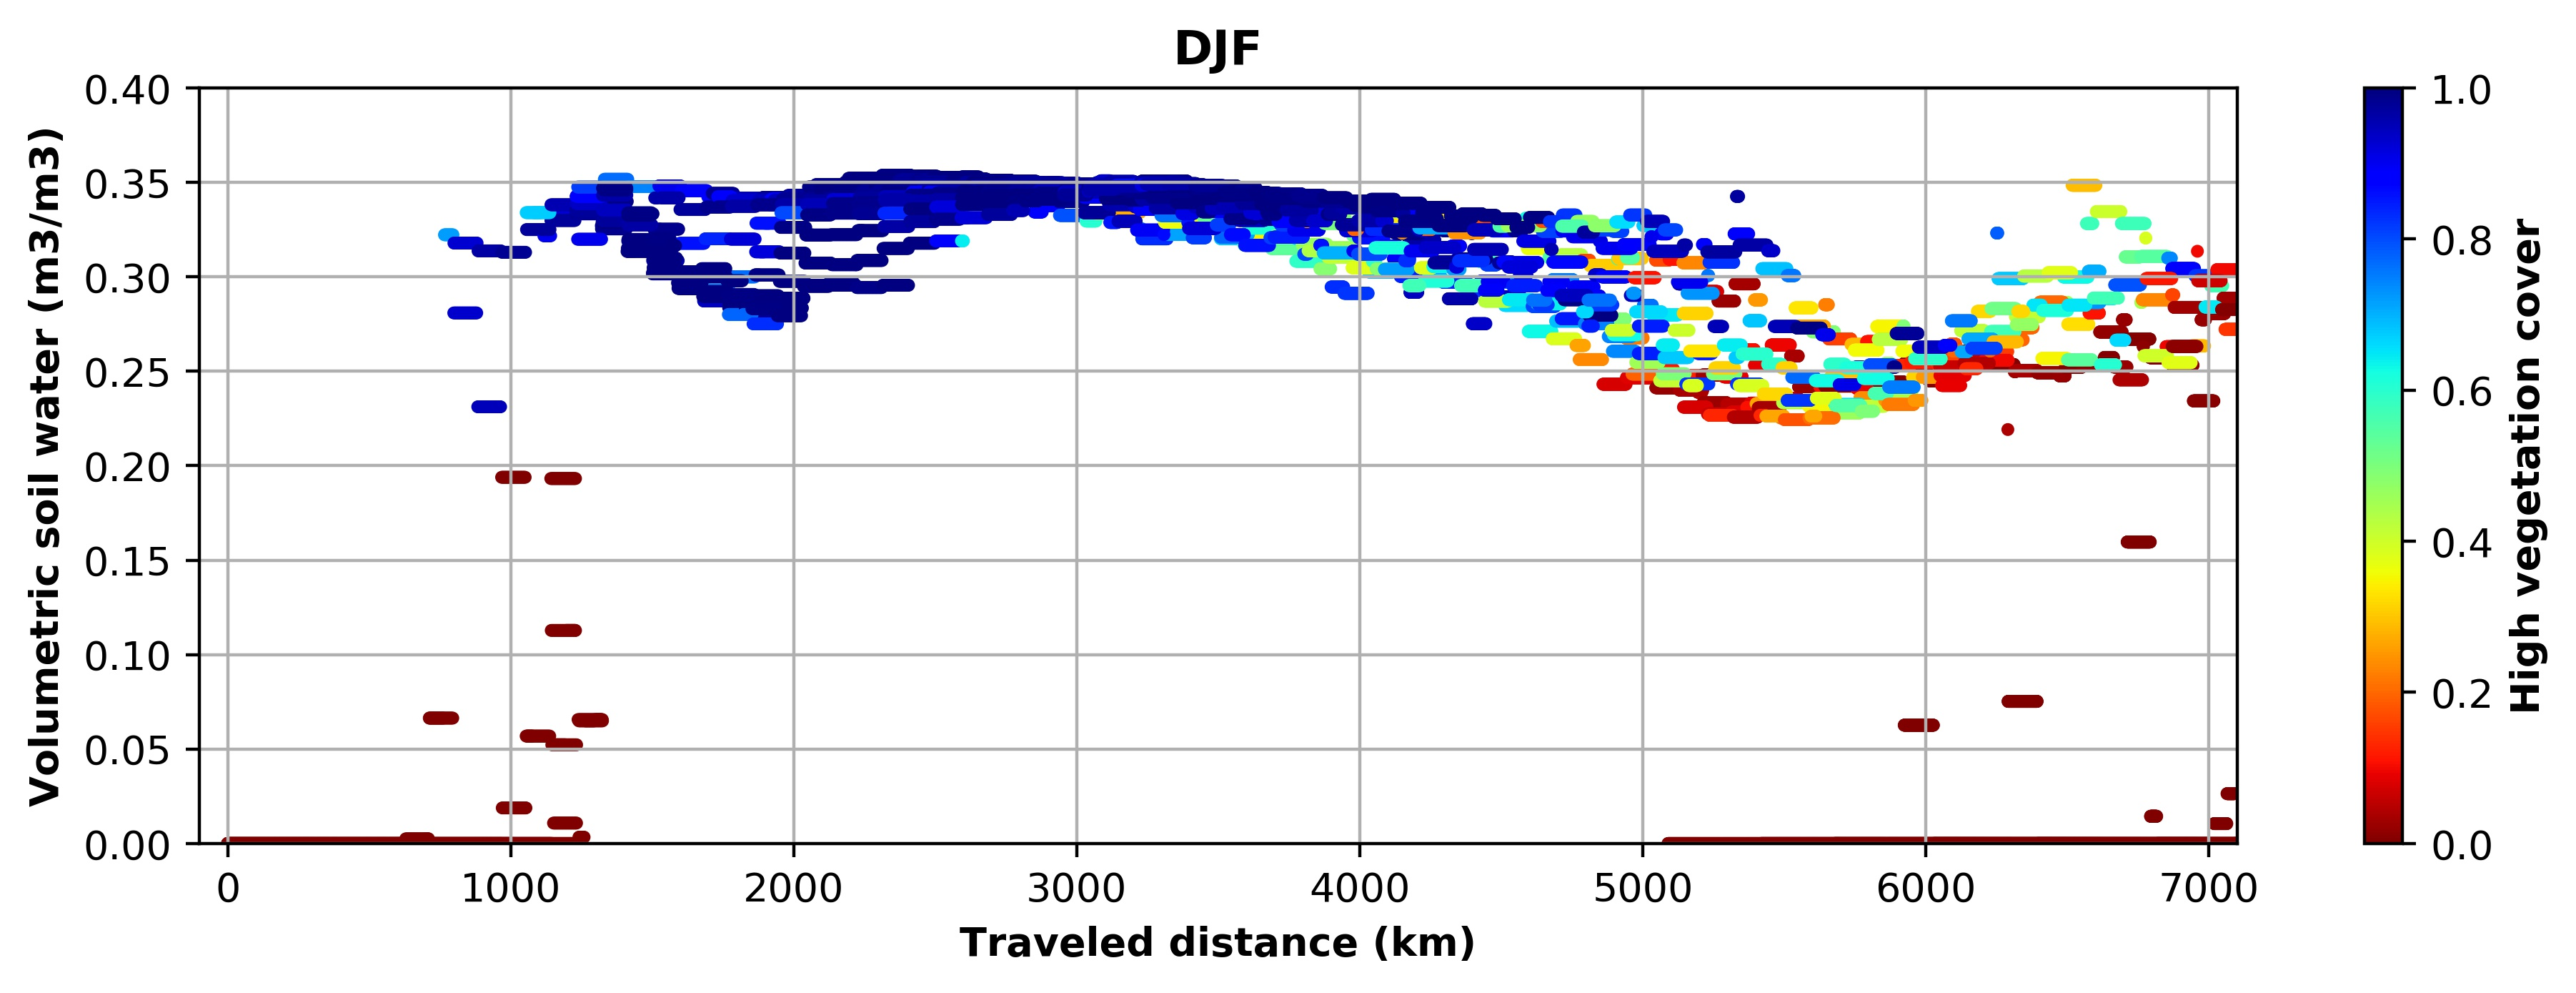
\includegraphics[width=0.49\linewidth]{VSDJF} 
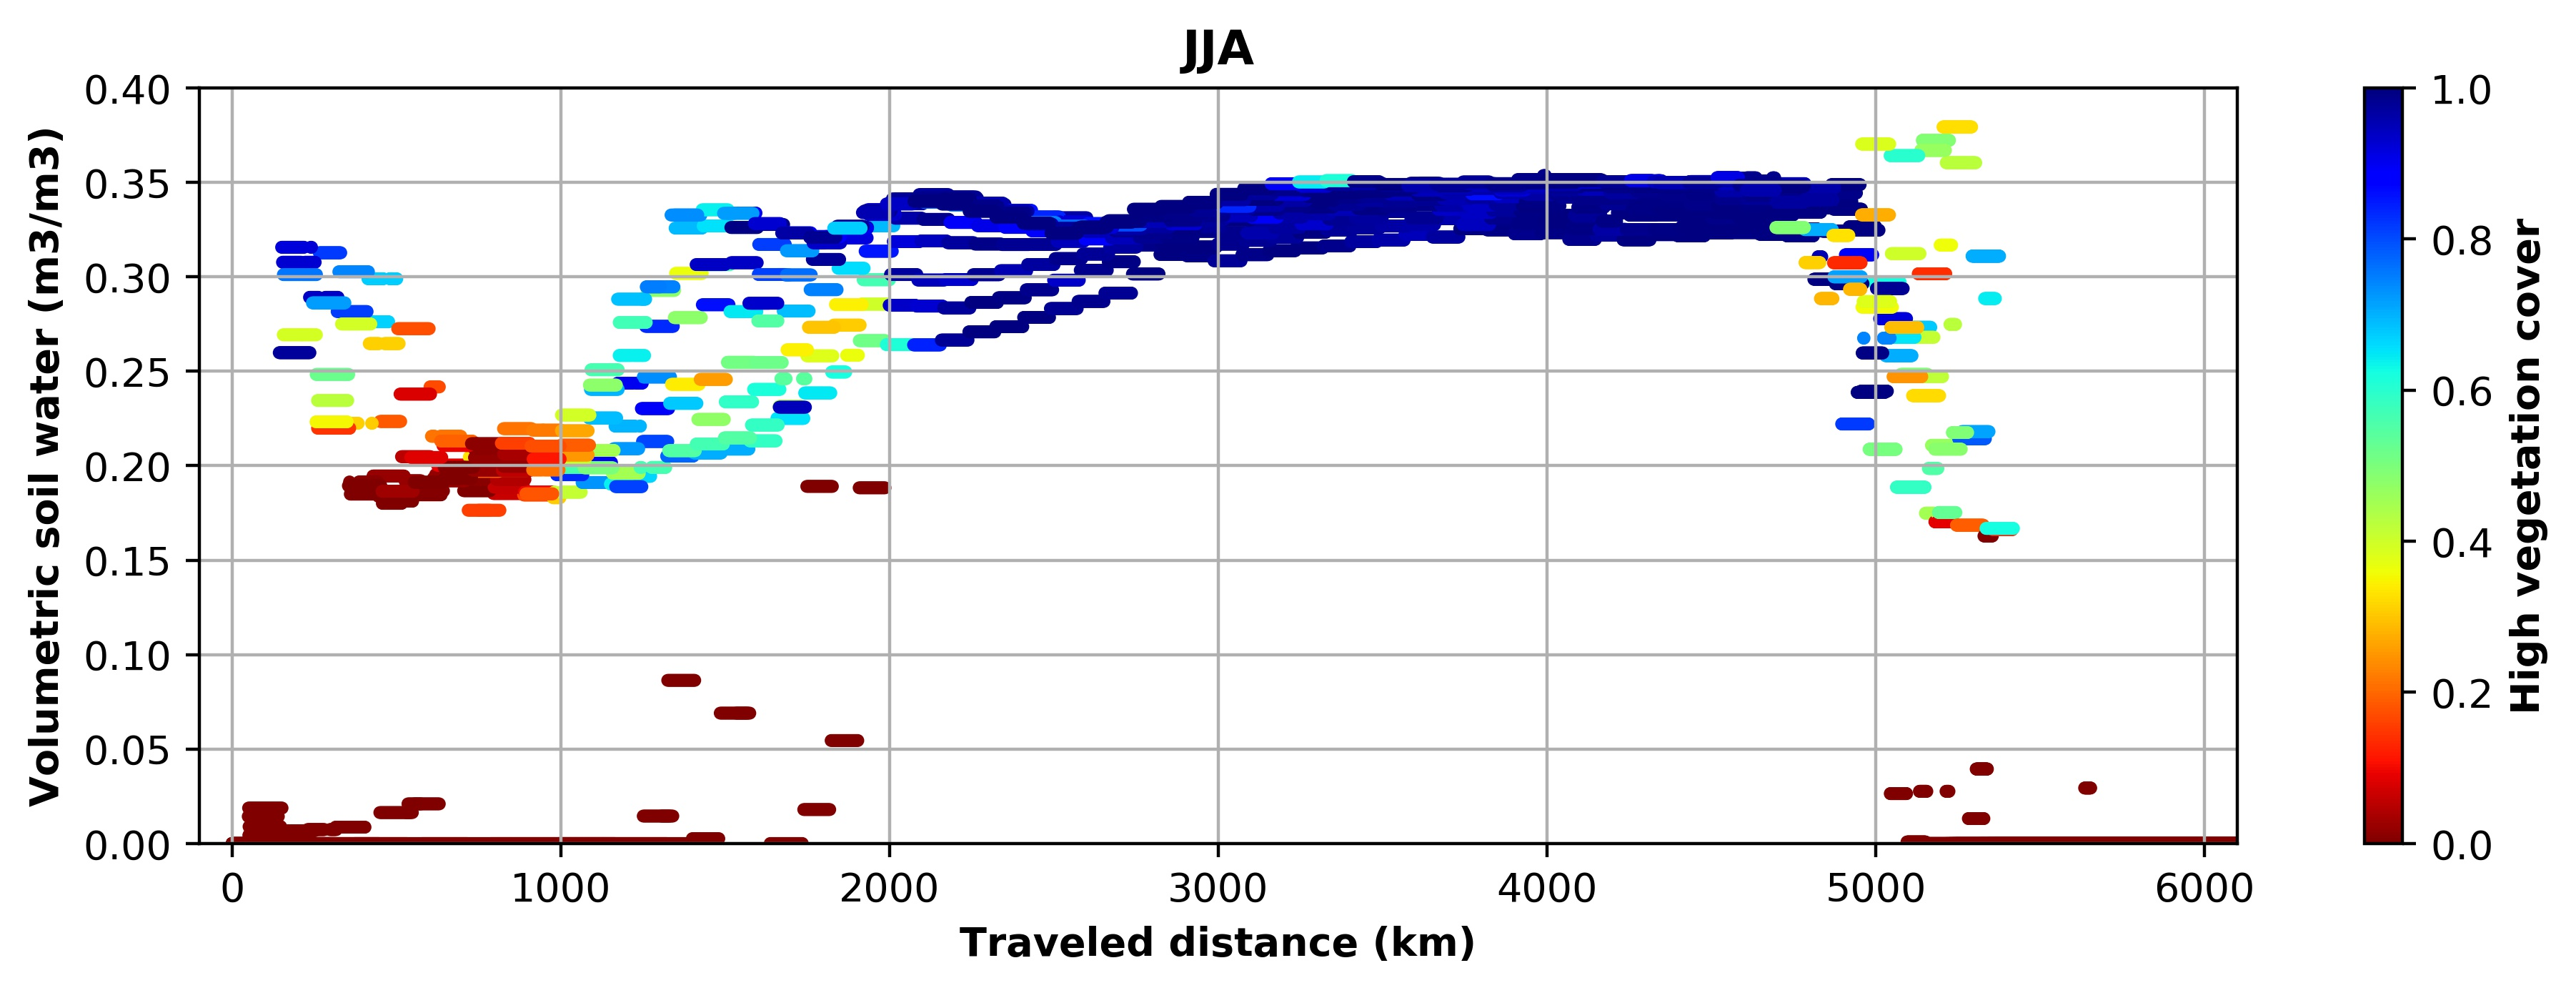
\includegraphics[width=0.49\linewidth]{VSJJA} 
\captionof{figure}{Seasonal means for the trajectories shown in Figure 1. The
figures on the left are the results for summer, and the ones on right are for
winter. From top to bottom row, we can see the results for precipitation,
evapotranspiration, precipitable water content, soil temperature, and volumetric
soil water.}
\end{center}

\end{multicols}
\end{document}